\documentclass[journal]{vgtc}                % final (journal style)
%\documentclass[review,journal]{vgtc}         % review (journal style)
%\documentclass[widereview]{vgtc}             % wide-spaced review
%\documentclass[preprint,journal]{vgtc}       % preprint (journal style)

%% Uncomment one of the lines above depending on where your paper is
%% in the conference process. ``review'' and ``widereview'' are for review
%% submission, ``preprint'' is for pre-publication, and the final version
%% doesn't use a specific qualifier.

%% Please use one of the ``review'' options in combination with the
%% assigned online id (see below) ONLY if your paper uses a double blind
%% review process. Some conferences, like IEEE Vis and InfoVis, have NOT
%% in the past.

%% Please note that the use of figures other than the optional teaser is not permitted on the first page
%% of the journal version.  Figures should begin on the second page and be
%% in CMYK or Grey scale format, otherwise, colour shifting may occur
%% during the printing process.  Papers submitted with figures other than the optional teaser on the
%% first page will be refused. Also, the teaser figure should only have the
%% width of the abstract as the template enforces it.

%% These few lines make a distinction between latex and pdflatex calls and they
%% bring in essential packages for graphics and font handling.
%% Note that due to the \DeclareGraphicsExtensions{} call it is no longer necessary
%% to provide the the path and extension of a graphics file:
%% 
\includegraphics{diamondrule} is completely sufficient.
%%
\ifpdf%                                % if we use pdflatex
  \pdfoutput=1\relax                   % create PDFs from pdfLaTeX
  \pdfcompresslevel=9                  % PDF Compression
  \pdfoptionpdfminorversion=7          % create PDF 1.7
  \ExecuteOptions{pdftex}
  \usepackage{graphicx}                % allow us to embed graphics files
  \DeclareGraphicsExtensions{.pdf,.png,.jpg,.jpeg} % for pdflatex we expect .pdf, .png, or .jpg files
\else%                                 % else we use pure latex
  \ExecuteOptions{dvips}
  \usepackage{graphicx}                % allow us to embed graphics files
  \DeclareGraphicsExtensions{.eps}     % for pure latex we expect eps files
\fi%

%% it is recomended to use ``\autoref{sec:bla}'' instead of ``Fig.~\ref{sec:bla}''
\graphicspath{{figures/}{pictures/}{images/}{./}} % where to search for the images

\usepackage{microtype}                 % use micro-typography (slightly more compact, better to read)
\PassOptionsToPackage{warn}{textcomp}  % to address font issues with \textrightarrow
\usepackage{textcomp}                  % use better special symbols
\usepackage{mathptmx}                  % use matching math font
\usepackage{times}                     % we use Times as the main font
\renewcommand*\ttdefault{txtt}         % a nicer typewriter font
\usepackage{cite}                      % needed to automatically sort the references
\usepackage{tabu}                      % only used for the table example
\usepackage{booktabs}                  % only used for the table example
%% We encourage the use of mathptmx for consistent usage of times font
%% throughout the proceedings. However, if you encounter conflicts
%% with other math-related packages, you may want to disable it.

%% In preprint mode you may define your own headline.
%\preprinttext{To appear in IEEE Transactions on Visualization and Computer Graphics.}

%% If you are submitting a paper to a conference for review with a double
%% blind reviewing process, please replace the value ``0'' below with your
%% OnlineID. Otherwise, you may safely leave it at ``0''.
\onlineid{0}

%% declare the category of your paper, only shown in review mode
\vgtccategory{Research}
%% please declare the paper type of your paper to help reviewers, only shown in review mode
%% choices:
%% * algorithm/technique
%% * application/design study
%% * evaluation
%% * system
%% * theory/model
\vgtcpapertype{VAST}

\title{Interactive Filter and Display of Hillary Clinton's Emails: \\A Cautionary Tale of Metadata}

\author{Christopher D. Salahub and R. Wayne Oldford}
\authorfooter{
%% insert punctuation at end of each item
\item
 Christopher D. Salahub, University of Waterloo, Canada \\E-mail: csalahub@uwaterloo.ca.
\item
 R. Wayne Oldford, University of Waterloo, Canada \\ E-mail: rwoldford@uwaterloo.ca.
}

%other entries to be set up for journal
\shortauthortitle{Salahub and Oldford: Filter and Display of Clinton's Emails}
%\shortauthortitle{Firstauthor \MakeLowercase{\textit{et al.}}: Paper Title}

\abstract{We present a web-based visualization that allows the user to interactively filter and display characteristics of 32,795 Hillary Clinton's emails as provided by Wikileaks.

The visualization focuses on the meta-data of each email, including its senders, receivers, and the timestamp the email appeared on the Clinton server.  An interactive time range slider filters all email and all displays automatically update to changes in the slider.  The main display shows Clinton's most frequent correspondents arranged as nodes of a spoked graph with Clinton at the centre.  Volume determines the thickness of each spoke and high volume determines an inner circle whose spokes are shortened.  Correspondents and their edges are coloured according to whether that email account could be identified as being an approved Federal government account or not.  A second display shows two daily time series: the total number of emails for that day, and the number meeting selection criteria.  A third display shows a scatterplot of the time of day versus the day on which that email appeared.  Scatterplot points are coloured by whether the email was redacted or not.  

Other displays add some information beyond metadata.  FOIA exemption codes appear as a selectable list and a barplot shows email counts by FOIA code.  The (stemmed) terms having highest frequency in the displayed email, and those having highest tf-idf are listed in separate displays.  All displays are interactively filtered by time range and selected FOIA codes.

We illustrate how the filtered displays can be used to generate hypotheses and uncover interesting information.  These touch on contentious issues including the handling of classified information, the 2012 attack on the Benghazi U.S. diplomatic compound, and emails apparently missing from those released publicly.  

The data are extracted from Wikileaks HTML files, cleaned, and stored in a form useful for interactive exploration.  A local \texttt{R} \texttt{shiny} server provides the interactive displays as a public service online tool to explore and uncover patterns in the meta-data and summary contents of Clinton's email.  Coupled with publicly available sources of information, these interactive tools uncover surprising amounts of information about an individual, especially one holding public office. The ease with which this can be accomplished and shared should serve as a clear warning as to what can be learned about anyone from metadata.
}

%% Keywords that describe your work. Will show as 'Index Terms' in journal
%% please capitalize first letter and insert punctuation after last keyword
\keywords{Exploratory data analysis, metadata, text mining, web-scraping, interactive web visualization,  \texttt{R},  \texttt{shiny} }

%% ACM Computing Classification System (CCS). 
%% See <http://www.acm.org/class/1998/> for details.
%% The ``\CCScat'' command takes four arguments.

\CCScatlist{ % not used in journal version
 \CCScat{K.6.1}{Management of Computing and Information Systems}%
{Project and People Management}{Life Cycle};
 \CCScat{K.7.m}{The Computing Profession}{Miscellaneous}{Ethics}
}

%% Uncomment below to include a teaser figure.
\teaser{
  \centering
  \begin{tabular}{cc}
  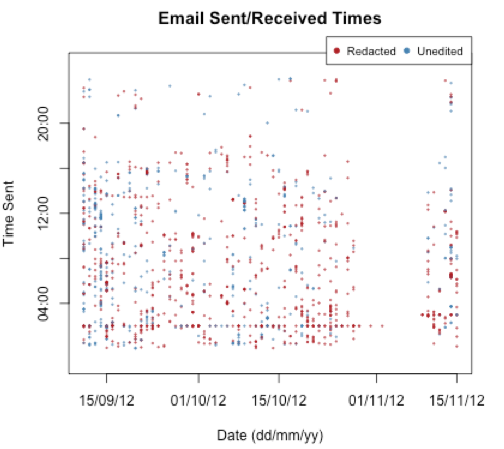
\includegraphics[width=0.25\textheight]{DailySept11ToNov152012_All} &
  \includegraphics[width=0.25\textheight]{InnerCircleSept11ToNov152012_All} \\
  &\\
  {\small (a) Missing data in November.} & {\small (b) Inner Circle: Correspondent info by colour; volume by thickness.}
  \end{tabular}
  \caption{Metadata: Time, date, correspondents, volume.  Filtered: Sept. 11 to Nov. 15, 2012.  
  %Source: \href{https://wikileaks.org/clinton-emails/}{\texttt{https://wikileaks.org/clinton-emails/}}
  }
  
	\label{fig:teaser}
}

%% Uncomment below to disable the manuscript note
%\renewcommand{\manuscriptnotetxt}{}

%% Copyright space is enabled by default as required by guidelines.
%% It is disabled by the 'review' option or via the following command:
% \nocopyrightspace

\vgtcinsertpkg

%%%%%%%%%%%%%%%%%%%%%%%%%%%%%%%%%%%%%%%%%%%%%%%%%%%%%%%%%%%%%%%%
%%%%%%%%%%%%%%%%%%%%%% START OF THE PAPER %%%%%%%%%%%%%%%%%%%%%%
%%%%%%%%%%%%%%%%%%%%%%%%%%%%%%%%%%%%%%%%%%%%%%%%%%%%%%%%%%%%%%%%%

\begin{document}
%% the only exception to this rule is the \firstsection command
\firstsection{Introduction}

\maketitle


The 2016 US Presidential election was one of the most contentious in history.  The existence and possible content of Hillary Clinton's private email server played an significant role in the campaign until the end. Despite their significant nature, very few of the individuals commenting on the significance of this server had spent any significant time viewing this content. This is no fault of theirs, the officially released data has previously only been stored in databases on the United States' State Department Website (see https://foia.state.gov/Learn/New.aspx) and Wikileaks (see https://wikileaks.org/clinton-emails/) in individually searchable form. Furthermore, the email data is stored in the inconvenient format of individual PDF documents, and in the case of Wikileaks a slightly more convenient but still cumbersome HTML representation based on the official PDF content. This granularity and separation of individual emails on different webpages prevents a great deal interesting analysis of the data, including any aggregate analyses of patterns in content or metadata. As such, the emails are incredibly misunderstood documents, and current searches for patterns and points of interest have relied upon searching for terms of interest and sifting through the results of the search. Such a method is not only tedious but problematic from a statistical point of view, as approaching any data set with a specific hypothesis before exploring its structure and patterns in abstract leads to biased conclusions and poor analysis. In the interest of simplifying the general exploration of this important data set, the Wikileaks HTML email versions were extracted and a series of visualizations were generated around the metadata included in these emails. An interactive web application in \texttt{R} \texttt{shiny} was constructed utilizing these visualizations and the extracted data. Incorporated in this app was a short article explaining the use of the app, providing links to background information, and outlining some of the findings of the more interesting trends observed. This framework provides any individual with interest the ability to generate hypotheses by exploring the data without necessarily searching for any particular conclusion. 

In generating and exploring this data, a considerable amount of respect is gained for the power of the often overlooked metadata of emails, especially with public figures. Simply having access to the network of communications, simple indicators of identifiable features of the individuals communicating, and times sent is enough to generate interesting questions which simple Google searches of important events and days can shed a great deal of light on. Leveraging data beyond this metadata, including the Freedom of Information Act (FOIA) exemption codes (see https://vault.fbi.gov/explanation-of-exemptions) used to redact the emails, only bolsters this simple metadata driven investigation. Metadata is often viewed as less significant or somehow less intrusive data, but the exploration performed in this paper demonstrated, at the very least to the authors, what a powerful tool metadata is for generating hypotheses about data. Given the lack of privacy present in the modern internet age and the amount of information most individuals make publicly available, there is a clear warning here about the utility of metadata for bad or for good. For a public official like Hillary Clinton, the data become even more interesting due to a number of contentious issues which arose during her tenure as the Secretary of State, independent of and as a result of her use of a private server.

\section{Data Extraction}

Before any of the analysis could begin, the emails had to be converted from the individual PDF and HTML form into a more easily used data structure. The choice was made to use the Wikileaks HTML emails as the source for data extraction. This choice was made primarily due to the relative ease of loading the raw HTML pages on the Wikileaks database due to their regular method of storage (the email with ID <id> is stored at https://wikileaks.org/clinton-emails/emailid/<id>) and ease of loading. These qualities made the HTML emails amenable to programmatic extraction, which was completed using a host of web-scraping and string parsing tools in \texttt{R}. In particular the packages \texttt{RCurl} and \texttt{XML} proved invaluable to extract the raw HTML pages for each email, and the packages \texttt{tm}, \texttt{stringr}, and \texttt{SnowballC} were indispensible to process and clean the raw HTML into a useable form. After downloading the raw HTML and extracting the data of interest, the resulting data was stored in csv files to provide the flexibility to load the data into any architecture or analysis tool desired.

Unfortunately, this data is not perfect. The PDF files released by the state department do not include the typical email server header with information about the time stamp inforamtion, the addresses of all involved, and other useful and regular information. Instead, these files appear more similar to screen captures of the emails, providing only the visual display a user would see without the useful information used to generate that display. As a result, the email addresses are occasionally not included, and there were initially concerns over the time zones used to generate the time stamp metadata. Furthermore, the HTML data on Wikileaks is frequently irregular in form, and although work has been done to make the cleaning and extraction functions as general as possible, there are still certainly fringe cases not considered which occur frequently enough to have an impact. It is also important to keep in mind the fact that the data have already been filtered twice. First by the emails chosen to be released by Clinton, and next by the emails and email sections which the State Department chose not to redact. Indeed, even the metadata can be affected by this redaction, as a number of individuals have their email addresses redacted in all communications, preventing certain analysis from being performed.

\section{Shiny App}

The app (HOST ADDRESS) provides the ability for users to place custom filters on the time frame of server time stamps and classification tags of the emails and view how a series of three displays change. The first of these is a spoked network graph of all corresponents with Clinton at the centre. The spokes are separated into two groups by the radial length of the spokes, these groups are determined automatically by the largest difference in volume of correspondence present in the data between the ordered counts of number of emails sent between individuals. As well, the width of the edges of the graph is determined by the volume of correspondence which occurred between Clinton and the correspondent in either direction. Finally, all edges and points are coloured according to a simple scheme. If the name associated with a node in the graph is at any point associated with an email address hosted at some '.gov' domain in the correspondences, they are coloured blue. Individuals with email addresses which are identifiably not hosted at a '.gov' domain are coloured red. Finally, individuals which cannot have their email host domain identified are coloured grey. It is important to note that for those individuals with grey spokes, the reason the email is not identifiable is the removal of the email by the state department. Such a redaction is not a guarantee that the email said individual used is not an official state email, but it is an indication that the email address is viewed as personal or private information, which suggests some email hosted outside of the '.gov' domain. Still, such speculation cannot be conclusively made, and so these emails are simply reported as they are, unidentifiable.

In addition to the spoked network graph, a time series plot of daily email volume is displayed. This plot has two lines, the first is a line showing the total volume of emails for each day, and the second shows the number of emails satisfying the classification filter criteria for a given day. This allows users to view which days have an exceptionally high or low number of classified conversations. Returning to the motivation of hypothesis generation, referencing world events on any days of interest provides a number of interesting insights on how public figures like Clinton react and respond to world events. To augment this graph, Clinton's official foreign visit schedule (https://history.state.gov/departmenthistory/travels/secretary/clinton-hillary-rodham) was extracted, cleaned, and incorporated into the application. This coloured time segments during which Clinton was travelling with blue rectangles, highlighting her pattern of foreign visits and allowing a comparison between these and the daily email sending patterns.

For an even more detailed view of exactly when emails are sent and what proportion are classified, a third plot of email sending times by day is included in the web application. This plot takes advantage of the time-stamps on every email and then plots the emails as points with times on the vertical axis and the day sent on the horizontal axis. The points in this scatterplot are then coloured according to whether the corresponding email was redacted, in which case the point is coloured red, or released in full, in which case the point is coloured blue. Alpha blending and transparency of these points was utilized to make the patterns present more obvious and prevent overplotting from obscuring any interesting results. 

Finally, a barplot of the FOIA exemption codes used in the selected data is displayed. It is important to notice that this barplot is not trivialized by the possibility of selecting individual FOIA exemption codes, as many of the emails in the data set are exempted on a number of grounds, and so have numerous FOIA exemption codes. Thus, this barplot is not only interesting when all codes are selected, but can be used to see which codes commonly co-occur in documents.

\section{Observations}

In designing, creating, testing, and playing with the app, a number of interesting observations were made. These are summarized below, and some address contentious issues in regards to Clinton's emails and a number of significant events which occurred during her tenure as the United States Secretary of State.

\subsection{Daily Email Patterns}

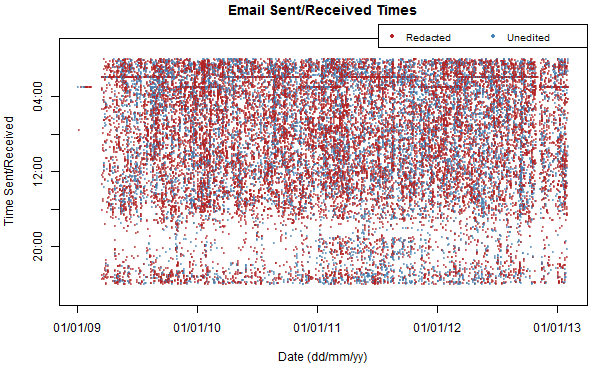
\includegraphics{SentReceivedEntireTenure}

The most striking thing noticed about the email sending times was the regularity of the pattern. Across the entirety of Clinton's four year tenure as the United States Secretary of State, email communication is densest between midnight and four in the morning, and there is a conspicuous gap in communication between roughly four in the afternoon and ten at night. This pattern is quite surprising, as it suggests that Clinton and her staff are most actively communicating late at night, rather than at the start of the regular work day around seven or eight in the morning. It would be expected that individuals would be sleeping late at night, and as a result that the density of emails would be relatively low. Rather, the data suggests that the only real break Clinton and her staff take from email communication is in the early evening, when many of them doubtless have official functions to attend. Regardless of the individual daily variation, the consistency of this pattern suggests that Clinton and her staff slept at strange times, and perhaps very irregularly, or were at least frequently interrupted by emails while sleeping. It is also possible these late night emails are more common because they are the ones Clinton chose to release, after all, it has been observed Clinton used the service Bleachbit to delete many old emails from her server (http://www.politico.com/story/2016/08/hillary-clinton-emails-bleachbit-227425, http://money.cnn.com/2016/08/26/technology/hillary-clinton-bleachbit/) and the organizational emails sent late at night to coordinate the following day may have simply been overlooked or maintained deliberately. Either way, the presence of such high volumes late at night tells a great deal about the irregularity of sleep that must have occurred among Clinton's staff during her tenure.

Another interesting pattern in the data is that of the two alternating modes at two and three in the morning. Immediately, hypothesizing that the cause of these modes is some regular server function is obvious due to the precision and consistency of the pattern. The alternation in the pattern was initially vexing, but comparing the shifts in the mode to the dates of daylight savings time in North America for the time period found a perfect match. It would seem that the alternation, then, is not deliberate, but rather a consequence of the one hour time shift that occurs in March and November every year in North America. Still, this observation does not reveal much about the content of the emails sent at this time, or why they are so regular. To better explore these emails, the app was run on a new set of data which was filtered to only contain the emails sent at two and three in the morning. Of the 32,359 emails sent during Clinton's tenure in this data set, 4,020 or roughly one eighth were sent at exactly two or three in the morning.

Historically important,  possibly had an impact on the 2016 US presidential election.

Contentious issues:
\begin{itemize}
\item private email server
\item classified documents (outside of state)
\item Sidney Blumenthal
\item Benghazi spin handling of media (Susan Rice)

\item scrubbing of her server (bleachbit)
\item missing email from online email State department
\end{itemize}


Learn:
\begin{itemize}
\item inner circle over time (state or not)
\item spike in email around Libyan revolution
\item gap in the email
\item daily email patterns, server behaviour (daylight savings time)
\end{itemize}

  
 Filter:
\begin{itemize}
\item time
\item redacted or not
\item FOIA exemption codes
\end{itemize}

   
 Content:
\begin{itemize}
\item Term frequency, TFIDF
\end{itemize}

   
 Tool: 
\begin{itemize}
\item Web-based, interactive filter and display tool
\end{itemize}
    
    
Discovery from visualization \& connecting discovery sources



- Nothing on this ... Preparation for Benghazi (security considerations)

- House Oversight and Government Reform Committee (standing committee) 
  Darrell Issa, Chair
     Jason Chaffetz, Chair (Gowdy a member)
  (discovered email server)
    ... 
- House Select Committee on Benghazi (Summer 2014) 
   Trey Gowdy, Chair

\section{Exposition}

Duis autem vel eum iriure dolor in hendrerit in vulputate velit esse
molestie consequat, vel illum dolore eu feugiat nulla facilisis at
vero eros et accumsan et iusto odio dignissim qui blandit praesent
luptatum zzril delenit augue duis dolore te feugait nulla
facilisi. Lorem ipsum dolor sit amet, consectetuer adipiscing elit,
sed diam nonummy nibh euismod tincidunt ut laoreet dolore magna
aliquam erat volutpat~\cite{Kindlmann:1999:SAG}.

\begin{equation}
\sum_{j=1}^{z} j = \frac{z(z+1)}{2}
\end{equation}

Lorem ipsum dolor sit amet, consetetur sadipscing elitr, sed diam
nonumy eirmod tempor invidunt ut labore et dolore magna aliquyam erat,
sed diam voluptua. At vero eos et accusam et justo duo dolores et ea
rebum. Stet clita kasd gubergren, no sea takimata sanctus est Lorem
ipsum dolor sit amet. Lorem ipsum dolor sit amet, consetetur
sadipscing elitr, sed diam nonumy eirmod tempor invidunt ut labore et
dolore magna aliquyam erat, sed diam voluptua. At vero eos et accusam
et justo duo dolores et ea rebum. Stet clita kasd gubergren, no sea
takimata sanctus est Lorem ipsum dolor sit amet.

\subsection{Lorem ipsum}

Lorem ipsum dolor sit amet (see \autoref{tab:vis_papers}), consetetur sadipscing elitr, sed diam
nonumy eirmod tempor invidunt ut labore et dolore magna aliquyam erat,
sed diam voluptua. At vero eos et accusam et justo duo dolores et ea
rebum. Stet clita kasd gubergren, no sea takimata sanctus est Lorem
ipsum dolor sit amet. Lorem ipsum dolor sit amet, consetetur
sadipscing elitr, sed diam nonumy eirmod tempor invidunt ut labore et
dolore magna aliquyam erat, sed diam voluptua. At vero eos et accusam
et justo duo dolores et ea rebum. Stet clita kasd gubergren, no sea
takimata sanctus est Lorem ipsum dolor sit amet. Lorem ipsum dolor sit
amet, consetetur sadipscing elitr, sed diam nonumy eirmod tempor
invidunt ut labore et dolore magna aliquyam erat, sed diam
voluptua. At vero eos et accusam et justo duo dolores et ea
rebum. 

\begin{table}[tb]
  \caption{VIS/VisWeek accepted/presented papers: 1990--2015.}
  \label{tab:vis_papers}
  \scriptsize%
	\centering%
  \begin{tabu}{%
	r%
	*{7}{c}%
	*{2}{r}%
	}
  \toprule
   year & \rotatebox{90}{Vis/SciVis} &   \rotatebox{90}{SciVis conf} &   \rotatebox{90}{InfoVis} &   \rotatebox{90}{VAST} &   \rotatebox{90}{VAST conf} &   \rotatebox{90}{TVCG @ VIS} &   \rotatebox{90}{CG\&A @ VIS} &   \rotatebox{90}{VIS/VisWeek} \rotatebox{90}{incl. TVCG/CG\&A}   &   \rotatebox{90}{VIS/VisWeek} \rotatebox{90}{w/o TVCG/CG\&A}   \\
  \midrule
  2015 & 33 & 9 & 38 & 33 & 14 & 17 & 15 & 159 & 127 \\
  2014 & 34 &   & 45 & 33 & 21 & 20 &   & 153 & 133 \\
  2013 & 31 &   & 38 & 32 &   & 20 &   & 121 & 101 \\
  2012 & 42 &   & 44 & 30 &   & 23 &   & 139 & 116 \\
  2011 & 49 &   & 44 & 26 &   & 20 &   & 139 & 119 \\
  2010 & 48 &   & 35 & 26 &   &   &   & 109 & 109 \\
  2009 & 54 &   & 37 & 26 &   &   &   & 117 & 117 \\
  2008 & 50 &   & 28 & 21 &   &   &   & 99 & 99 \\
  2007 & 56 &   & 27 & 24 &   &   &   & 107 & 107 \\
  2006 & 63 &   & 24 & 26 &   &   &   & 113 & 113 \\
  2005 & 88 &   & 31 &   &   &   &   & 119 & 119 \\
  2004 & 70 &   & 27 &   &   &   &   & 97 & 97 \\
  2003 & 74 &   & 29 &   &   &   &   & 103 & 103 \\
  2002 & 78 &   & 23 &   &   &   &   & 101 & 101 \\
  2001 & 74 &   & 22 &   &   &   &   & 96 & 96 \\
  2000 & 73 &   & 20 &   &   &   &   & 93 & 93 \\
  1999 & 69 &   & 19 &   &   &   &   & 88 & 88 \\
  1998 & 72 &   & 18 &   &   &   &   & 90 & 90 \\
  1997 & 72 &   & 16 &   &   &   &   & 88 & 88 \\
  1996 & 65 &   & 12 &   &   &   &   & 77 & 77 \\
  1995 & 56 &   & 18 &   &   &   &   & 74 & 74 \\
  1994 & 53 &   &   &   &   &   &   & 53 & 53 \\
  1993 & 55 &   &   &   &   &   &   & 55 & 55 \\
  1992 & 53 &   &   &   &   &   &   & 53 & 53 \\
  1991 & 50 &   &   &   &   &   &   & 50 & 50 \\
  1990 & 53 &   &   &   &   &   &   & 53 & 53 \\
  \midrule
  \textbf{sum} & \textbf{1515} & \textbf{9} & \textbf{595} & \textbf{277} & \textbf{35} & \textbf{100} & \textbf{15} & \textbf{2546} & \textbf{2431} \\
  \bottomrule
  \end{tabu}%
\end{table}

\subsection{Mezcal Head}

Lorem ipsum dolor sit amet (see \autoref{fig:sample}), consetetur sadipscing elitr, sed diam
nonumy eirmod tempor invidunt ut labore et dolore magna aliquyam erat,
sed diam voluptua. At vero eos et accusam et justo duo dolores et ea
rebum. Stet clita kasd gubergren, no sea takimata sanctus est Lorem
ipsum dolor sit amet. Lorem ipsum dolor sit amet, consetetur
sadipscing elitr, sed diam nonumy eirmod tempor invidunt ut labore et
dolore magna aliquyam erat, sed diam voluptua. At vero eos et accusam
et justo duo dolores et ea rebum. Stet clita kasd gubergren, no sea
takimata sanctus est Lorem ipsum dolor sit amet. 

\subsubsection{Duis Autem}

Lorem ipsum dolor sit amet, consetetur sadipscing elitr, sed diam
nonumy eirmod tempor invidunt ut labore et dolore magna aliquyam erat,
sed diam voluptua. At vero eos et accusam et justo duo dolores et ea
rebum. Stet clita kasd gubergren, no sea takimata sanctus est Lorem
ipsum dolor sit amet. Lorem ipsum dolor sit amet, consetetur
sadipscing elitr, sed diam nonumy eirmod tempor invidunt ut labore et
dolore magna aliquyam erat, sed diam voluptua. At vero eos et accusam
et justo duo dolores et ea rebum. Stet clita kasd gubergren, no sea
takimata sanctus est Lorem ipsum dolor sit amet. Lorem ipsum dolor sit
amet, consetetur sadipscing elitr, sed diam nonumy eirmod tempor
invidunt ut labore et dolore magna aliquyam erat, sed diam
voluptua. At vero eos et accusam et justo duo dolores et ea
rebum. Stet clita kasd gubergren, no sea takimata sanctus est. Lorem
ipsum dolor sit amet.

\begin{figure}[tb]
 \centering % avoid the use of \begin{center}...\end{center} and use \centering instead (more compact)
 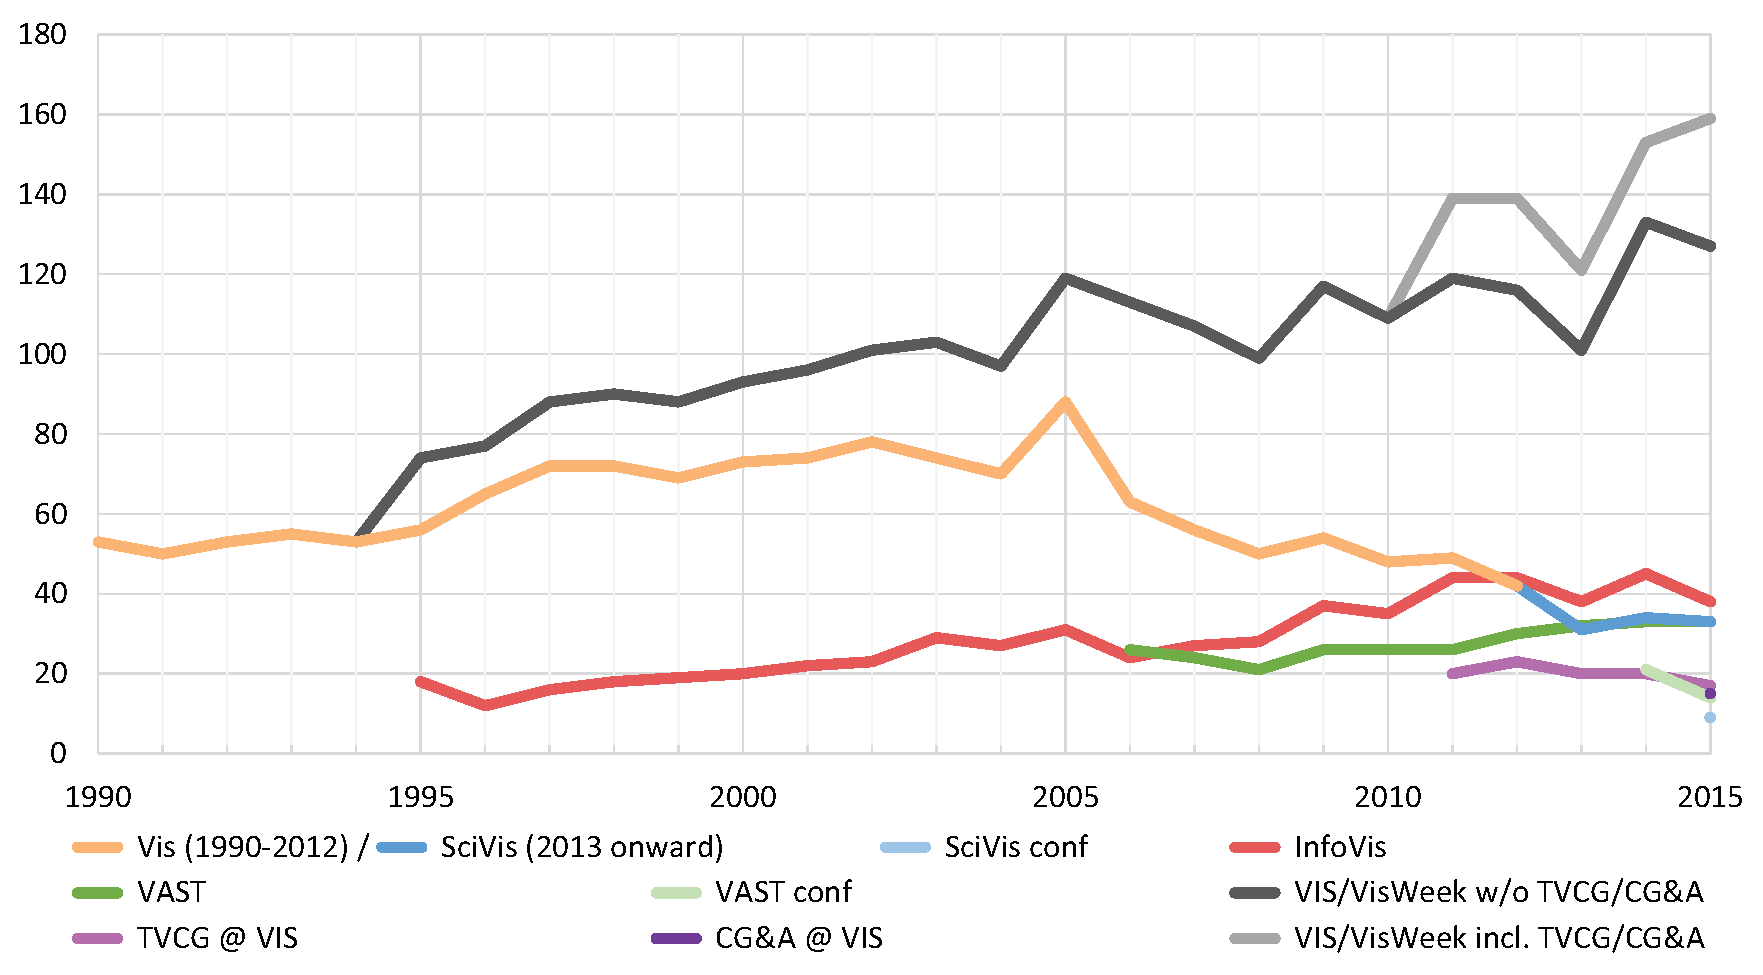
\includegraphics[width=\columnwidth]{paper-count-w-2015-new}
 \caption{A visualization of the data from \autoref{tab:vis_papers}. The image is from \cite{Isenberg:2017:VMC} and is in the public domain.}
 \label{fig:sample}
\end{figure}

\subsubsection{Ejector Seat Reservation}

Duis autem~\cite{Lorensen:1987:MCA}\footnote{The algorithm behind
Marching Cubes \cite{Lorensen:1987:MCA} had already been
described by Wyvill et al. \cite{Wyvill:1986:DSS} a year
earlier.} vel eum iriure dolor in hendrerit
in vulputate velit esse molestie consequat,\footnote{Footnotes
appear at the bottom of the column.} vel illum dolore eu
feugiat nulla facilisis at vero eros et accumsan et iusto odio
dignissim qui blandit praesent luptatum zzril delenit augue duis
dolore te feugait nulla facilisi. Lorem ipsum dolor sit amet,
consectetuer adipiscing elit, sed diam nonummy nibh euismod tincidunt
ut laoreet dolore magna aliquam erat volutpat.


\paragraph{Confirmed Ejector Seat Reservation}

Ut wisi enim ad minim veniam, quis nostrud exerci tation ullamcorper
suscipit lobortis nisl ut aliquip ex ea commodo
consequat~\cite{Nielson:1991:TAD}. Duis autem vel eum iriure dolor in
hendrerit in vulputate velit esse molestie consequat, vel illum dolore
eu feugiat nulla facilisis at vero eros et accumsan et iusto odio
dignissim qui blandit praesent luptatum zzril delenit augue duis
dolore te feugait nulla facilisi.

\paragraph{Rejected Ejector Seat Reservation}

Ut wisi enim ad minim veniam, quis nostrud exerci tation ullamcorper
suscipit lobortis nisl ut aliquip ex ea commodo consequat. Duis autem
vel eum iriure dolor in hendrerit in vulputate velit esse molestie


\section{Conclusion}

Lorem ipsum dolor sit amet, consetetur sadipscing elitr, sed diam
nonumy eirmod tempor invidunt ut labore et dolore magna aliquyam erat,
sed diam voluptua. At vero eos et accusam et justo duo dolores et ea
rebum. Stet clita kasd gubergren, no sea takimata sanctus est Lorem
ipsum dolor sit amet. Lorem ipsum dolor sit amet, consetetur
sadipscing elitr, sed diam nonumy eirmod tempor invidunt ut labore et
dolore magna aliquyam erat, sed diam voluptua. At vero eos et accusam
et justo duo dolores et ea rebum. Stet clita kasd gubergren, no sea
takimata sanctus est Lorem ipsum dolor sit amet. Lorem ipsum dolor sit
amet, consetetur sadipscing elitr, sed diam nonumy eirmod tempor
invidunt ut labore et dolore magna aliquyam erat, sed diam
voluptua. At vero eos et accusam et justo duo dolores et ea
rebum.


%% if specified like this the section will be committed in review mode
\acknowledgments{
The authors wish to thank A, B, C. This work was supported in part by
a grant from XYZ.}

%\bibliographystyle{abbrv}
\bibliographystyle{abbrv-doi}
%\bibliographystyle{abbrv-doi-narrow}
%\bibliographystyle{abbrv-doi-hyperref}
%\bibliographystyle{abbrv-doi-hyperref-narrow}

\bibliography{template}

\end{document}
